\section{A desciption of the data set}

The dataset is composed by an examination of Pima Indians in Phoenix, Arizona.
They were chosen as subject due to their high risk of getting diabetes.
The dataset was used as a way to predict if Indian women could develop diabetes in the following 5 years.
The examination had picked out a number of attributes which they found relevant to the examination.
The data was picked out by: “Jack W. Smith, et al., 1988, Using the ADAP Learning Algorithm to Forecast the Onset of Diabetes Mellitus”
and is taken from a bigger examination made by “National Institute of Diabetes and Digestive and Kidney Diseases.”
The dataset contains 8 attributes, plus a class attribute which identifies whether or not the person was tested positive for diabetes,
 and the test was taken by 768 test subjects.

The dataset is composed by the following attributes:
\begin{enumerate}
\item Number of times pregnant
\item Plasma glucose concentration a 2 hours in an oral glucose tolerance test, GTT
\item Diastolic blood pressure (mm Hg)
\item Triceps skin fold thickness (mm)
\item 2-Hour serum insulin ($\mu$ U / ml)
\item Body mass index Weight in (kg / (Height in $m^2$))
\item Diabetes pedigree function
\item Age (Years)

\item \emph{class attribute}:
\item Class variable (0 or 1)
\end{enumerate}


The dataset was found on the website: (http://archive.ics.uci.edu/ml/datasets/Pima%20Indians%20Diabetes)
In the folder "Data Folder".

The obvious variable to predict
in any sort of supervised learning scenario
is the class attribute,
as it distinguishes between
those patients with diabetes and those without.
A classification would be the simplest,
and easy for an end user,
but with a regression
we can include our confidence in the diagnosis
despite the class variable being discrete.

As the data contains a multitude of missing values,
an important first step would be to clean it up.
A ``safe'' way to do so would be to simply remove any data points
with missing values,
assuming that there is no systematic bias
which would cause missing values for certain patients.

As for the unsupervised case,
the data might reasonably be expected to have certain correlations
and groupings
which might be exploited
in order to identify different clusters.
For example, older women will have a higher chance of having had more children,
simply due to having had more time to have them,
and with skin fold thickness and BMI both being measures of potential obesity,
they might be expected to correlate.
Due to the lack of discrete (TODO binary? set-membership, maybe?) variables,
an association mining as such cannot be supported on this data,
but some of the concepts might be generalizable to a continous case.

After taking into account the difference between healthy and diabetic patients,
an anomaly detection might perhaps be of the most use in identifying
potential data quality issues.

\section{A detailed explanation of the attributes of the data.}

This dataset contains 8 attributes which work as input. These attributes are defined in
the above section and are discussed more in depth in the following.

The number of times pregnant is a discrete ratio attribute and so is
the age attribute. Both attributes are measured in a finite set of values.
Plasma glucose concentration is a continuous ratio attribute
and so is diastolic blood pressure, skin fold thickness, BMI and 2-hour serum and
insulin. This means that only one of the eight input attributes is non-ratio.
The diabetes pedigree function is a continous ordinal attribute, because these
numbers tell whether one is more or less genetically expected to be diagnosed
with diabetes. Here, a value of 0 does not clearly mean an absence of the attribute.
Some of the attributes are continous by nature but appear as integers in the dataset.
For this reason, they have been classified as continous here despite having been written
down as integers in the dataset. This applies for the attributes bmi, insulin,
thickness, bp and glucose.
\bigskip

\begin{description}
\item [Number of times pregnant] Discrete ratio
\item [Plamsa glucose concentration] Continous ratio
\item [Diastolic blood pressure] Continous ratio
\item [Triceps skin fold] Continous ratio
\item [2-Hour serum insulin] Continous ratio
\item [Body mass index (BMI)] Continous ratio
\item [Diabetes pedigree function] Continous ordinal
\item [Age] Discrete ratio
\end{description}


Some of the recorded data make no biological sense and observations with one or
more nonsense values in its attributes have been discarded from the dataset.
Common sense has been applied to filter out obviously foul observations, such
as entries that dictate concentrations of blood plasma glucose to be zero, blood
pressure of zero, skin fold thickness as zero or BMI of zero. This means a
considerable amount of the original observations have been discarded, as the
data set went from 768 observations to 392.
\bigskip

Some summary statistics have been summarized in the tables below in Table 1. This should
give some insight to the values usually seen in the attributes. Mean, variance
and correalation have been presented for the attributes. Here, the huge differences
in the variance of the attributes should be noted. Some are very high, some are
almost non-existent.

\begin{table}[]
\centering
\caption{Mean and median of attributes}
\label{tab:stats}
\begin{tabular}{lllllllll}
\cline{1-1}
\multicolumn{1}{|l|}{Attribute} & pregs & glucose & bp   & thickness & insulin & bmi  & dia\_pedig & age  \\ \cline{1-1}
\multicolumn{1}{|l|}{Mean}      & 3.3   & 122.6   & 70.7 & 29.1      & 156.1   & 33.0 & 0.5        & 30.9 \\ \cline{1-1}
\multicolumn{1}{|l|}{Variance}  & 10.3     & 950.0     & 155.8   & 110.3        & 14087.3    & 49.3 & 0.1       & 103.8 \\ \cline{1-1}
                                                       &       &         &      &           &         &      &            &      \\ \hline
\end{tabular}
\end{table}

\begin{table}
\caption{Correalation matrix}
\label{tab:cor}
\begin{tabular}{lrrrrrrrrr}
{} &  pregs &  glucose &    bp &  thickness &  insulin &   bmi &  dia\_pedig &   age &  class \\
\midrule
pregs     &   1.00 &     0.20 &  0.21 &       0.09 &     0.08 & -0.03 &       0.01 &  0.68 &   0.26 \\
glucose   &   0.20 &     1.00 &  0.21 &       0.20 &     0.58 &  0.21 &       0.14 &  0.34 &   0.52 \\
bp        &   0.21 &     0.21 &  1.00 &       0.23 &     0.10 &  0.30 &      -0.02 &  0.30 &   0.19 \\
thickness &   0.09 &     0.20 &  0.23 &       1.00 &     0.18 &  0.66 &       0.16 &  0.17 &   0.26 \\
insulin   &   0.08 &     0.58 &  0.10 &       0.18 &     1.00 &  0.23 &       0.14 &  0.22 &   0.30 \\
bmi       &  -0.03 &     0.21 &  0.30 &       0.66 &     0.23 &  1.00 &       0.16 &  0.07 &   0.27 \\
dia\_pedig &   0.01 &     0.14 & -0.02 &       0.16 &     0.14 &  0.16 &       1.00 &  0.09 &   0.21 \\
age       &   0.68 &     0.34 &  0.30 &       0.17 &     0.22 &  0.07 &       0.09 &  1.00 &   0.35 \\
class     &   0.26 &     0.52 &  0.19 &       0.26 &     0.30 &  0.27 &       0.21 &  0.35 &   1.00 \\
\bottomrule
\end{tabular}
\end{table}

\section{Data Visualization}

\subsection{Visualizing the data}
!!3.1!!
We made a boxplot analysis, Figure \ref{fig:hists}, and it showed clearly that attribute 5(insulin) had the most outliers
and had the greatest variance. Attribute 2(glucose) had the second greatest variance but had no outliers.
All though the plots showed a lot of outliers for the attribute insulin, we did not remove them because we
assume that the examination was performed and measured correctly.
All of the attributes' boxplots have the same y-axes. This detail is important because each attribute describes a
biological factor, which vary greatly in value.
For example attribute 1(pregs) there is not a high variance. This could be because of the Indian women not having
a great amount of children, which is normal.

\begin{figure}
  \centering{}
  \caption{TODO caption}\label{fig:hists}
  \begin{subfigure}{0.3\textwidth}
    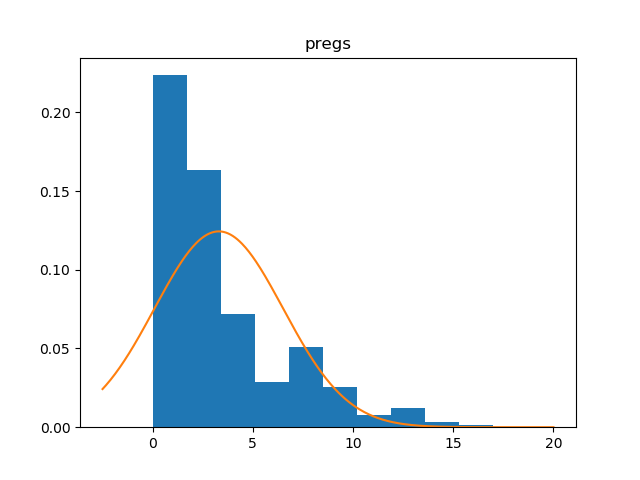
\includegraphics[width=\textwidth]{pregs_hist}
    \caption{TODO caption pregs}
  \end{subfigure}
  \begin{subfigure}{0.3\textwidth}
    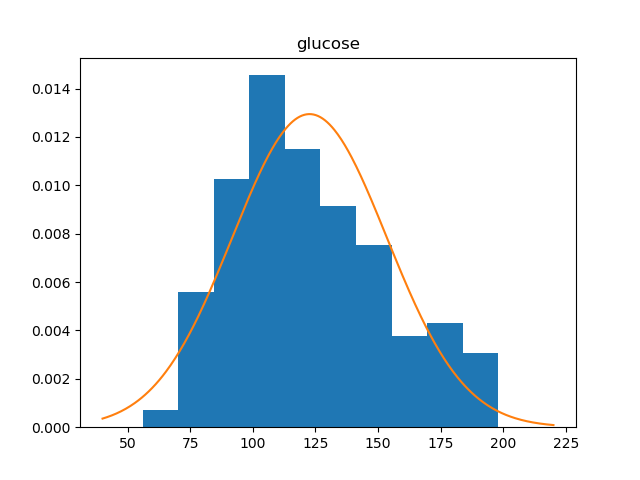
\includegraphics[width=\textwidth]{glucose_hist}
    \caption{TODO caption glucose}
  \end{subfigure}
  \begin{subfigure}{0.3\textwidth}
    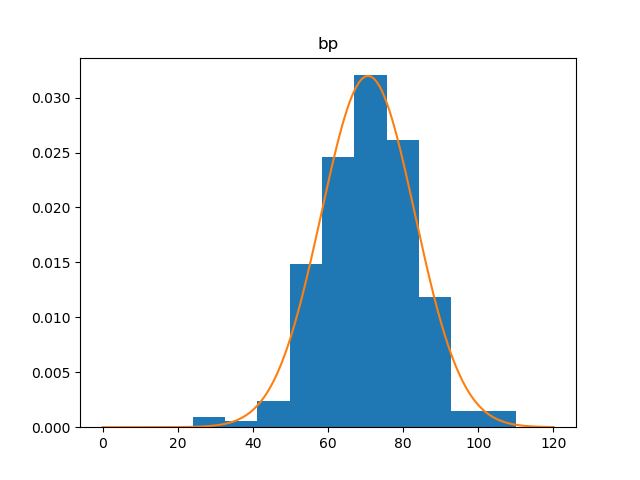
\includegraphics[width=\textwidth]{bp_hist}
    \caption{TODO caption bp}
  \end{subfigure}

  \begin{subfigure}{0.3\textwidth}
    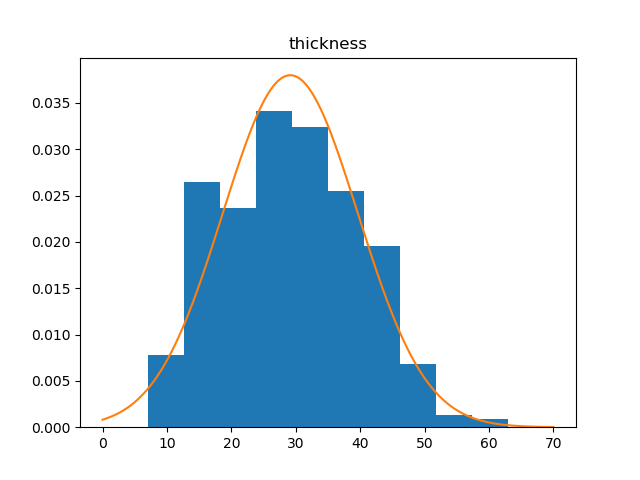
\includegraphics[width=\textwidth]{thickness_hist}
    \caption{TODO caption thickness}
  \end{subfigure}
  \begin{subfigure}{0.3\textwidth}
    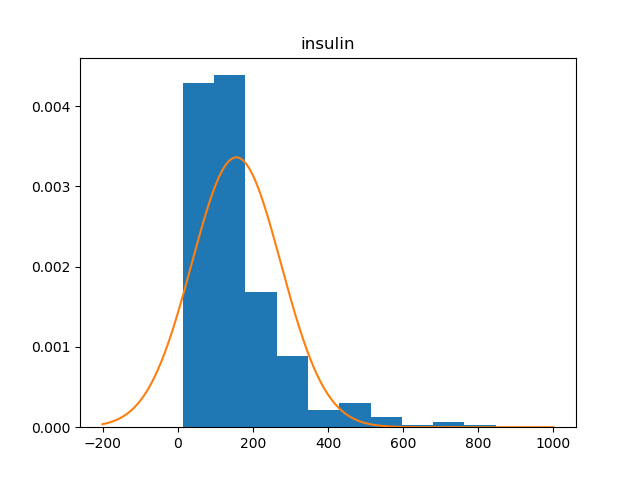
\includegraphics[width=\textwidth]{insulin_hist}
    \caption{TODO caption }
  \end{subfigure}
  \begin{subfigure}{0.3\textwidth}
    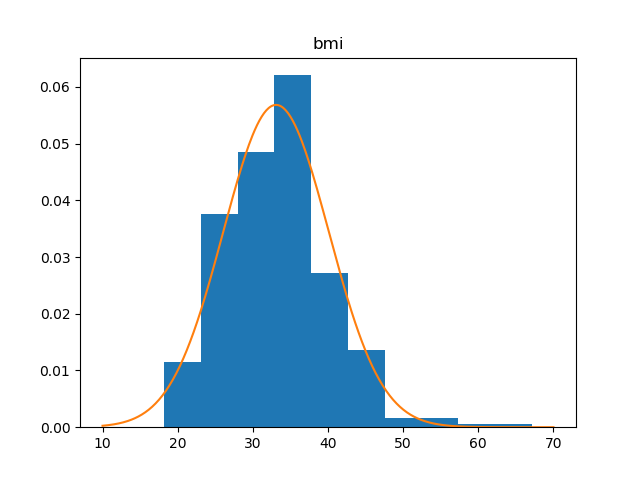
\includegraphics[width=\textwidth]{bmi_hist}
    \caption{TODO caption bmi}
  \end{subfigure}

  \begin{subfigure}{0.3\textwidth}
    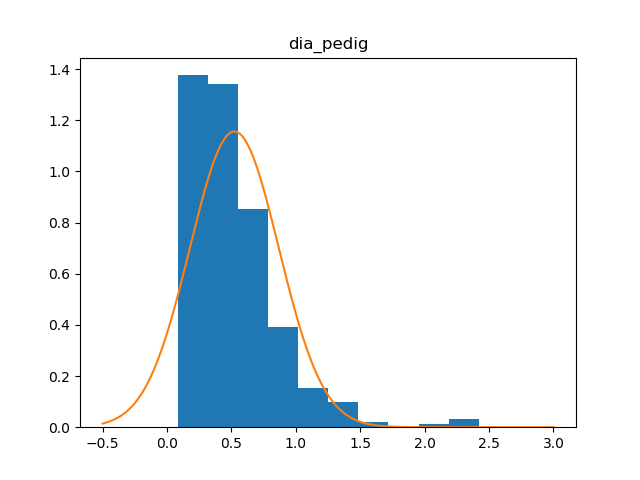
\includegraphics[width=\textwidth]{dia_pedig_hist}
    \caption{TODO caption dia\_pedig}
  \end{subfigure}
  \begin{subfigure}{0.3\textwidth}
    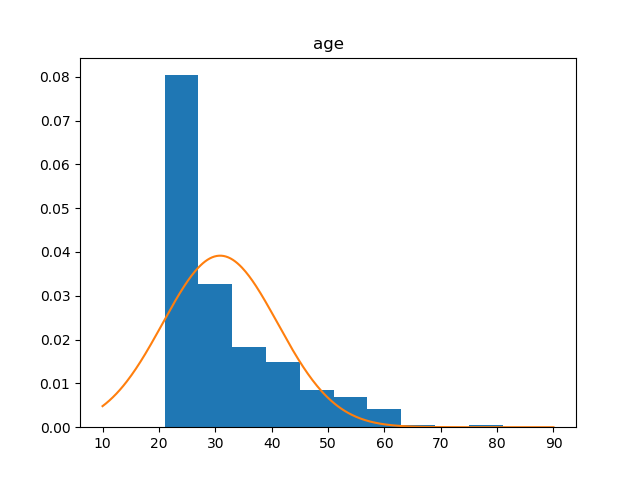
\includegraphics[width=\textwidth]{age_hist}
    \caption{TODO caption age}
  \end{subfigure}
  \begin{subfigure}{0.3\textwidth}
    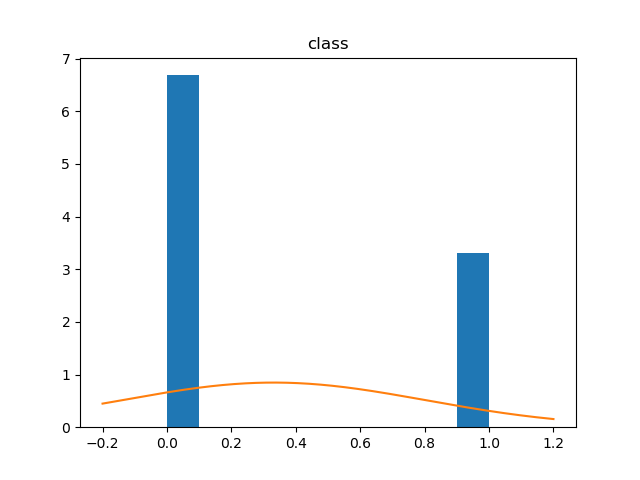
\includegraphics[width=\textwidth]{class_hist}
    \caption{TODO caption class}
  \end{subfigure}
\end{figure}

!!3.2!!
Histograms are shown in Figure \ref{fig:hists}. The attributes pregs, insulin, dia\_pedig
and age do not seem normal distributed. Bp seems to be normally distributed.
The data's attributes seem to be either right- or left-skewed, for example insulin and pregs
are both right-skewed. Bmi may seem to be normally distributed but has a
heavy tails to the right.
Overall the data seems quite non-normally distributed with a few exceptions as mentioned above.

!!3.3!!
The linear correlations of the non-standardized data are show in Table 2.
The higest correlation constant by far is the pregs-age one, which suggests
that observations with a high value in one of these entries will be more likely
to also have a high value in the other, quite as anticipated. This translates to
an apparent tendency for older women to have been pregnant more and for women
who have been pregnant more often to be older.
BMI and thickness seem to be correlated about as much as pregs and age. This
correlation seems reasonable as well.

!!3.4!!
The primary modelling aim, to predict whether an Indian woman has diabetes or not
based on 8 variables, appears to be feasible. However, given the nature of the
data, PCA will most likely not give a complete picture between these variables
and the occurrence of diabetes. It is very likely that the high variance of
insulin will outshine everything else, at least with the non-standardized
data. The PCA is designed this way, and it must be kept in mind that great
variation might not equal great importance.
The modelling of this data seems to be doable, but with what is known about the data
so far, it is hard to tell how much insight this will lead to.

\subsection{Visualizing the data with PCA}

The PCA revealed that a lot of the variance in the data is described by the
first principal component, the insulin. This principal component accounts for
93% of the total variance, and together with the second principal component, 97% of
the variance in the data is explained. This means a lot of the variance can
be described in a 2D-plot. A cumulative sum can be seen on figure (TODO ?? "cum.var.png") as a
function of principal components, from principal component describing the most
variance to the principal component describing the least variance. This is true
when the data is not standardized. However, after standardization, the variance
cannot be explained by one or two principle components, and therefore visualization
in 2D or even 3D becomes hard without loss of information about the data. See figure
(TODO ?? "exp\_var\_hist.png") for an overview of the explained variance for each principal component.

When the data is not standardized, the principal component with the most
responsibility for the variance in the dataset is, by far, insulin. Therefore,
this is more or less the first principal direction in which we plot our data. The second
principal direction is much dictated by the attribute glucose, which is the
attribute with the second highest variance. In this way, the projected plot in
2D can more or less (but, of course, not entirely) be thought of as
projection of the data down to the plane in the insulin and glucose directions.
Figure (TODO ?? "principal\_directions.png") shows in which direction the principal components point. The "spikes"
in each graph show how the principal directions point mostly in the direction of
insulin and glucose (indexed 1 and 4), respectively. After standardization, the principal
directions align much less with any principal components, which does make sense
considering how the variance had to be presented by more principal components
after standardization. This is visualized in figure (TODO ?? "principal\_directions\_n.png").
It is seen that now, the second principal direction points a bit more in the direction
of age and pregs, which also had a somewhat high correlation.

Here, the data can be seen projected to the principal components non-standardized
(TODO ?? "PCA.png") and standardized (TODO ?? "PCA\_n.png")

\section{Discussion}
As we saw in the normalized PCA and the correlation matrix,
there is little in the way of clear
linear relationships that account for
large amounts of the variance of the dataset.
The un-normalized PCA was dominated by a few high-variance attributes.
This indicates that we might rather want to perform a factor analysis,
as that method focuses on explaining the covariances between factors rather
than the overall variance of dthe dataset.

Another challenge,
especially for PCA,
is that the attributes are of wildly varying scales
with a range of 832 for insulin compared to merely 2.3
for the diabetes pedigree function.

The projections of the data into lower-dimensional spaces
initially seems to have a discouraging lack of the sort structure
one might expect would make unsupervised learning techniques like clustering useful.
However, including the class variable reveals structure in the data
that indicate it might still be amenable to
the supervised learning of a predictor.

We saw a number of correlations in the data,
including, as expected,
between age and number of times pregnant,
and bmi and skin thickness,
but also between blood glucose levels and insulin after a glucose tolerance test,
and generally between a cluster of attributes corresponding to
the (stereo)typical diabetes type 2 patient.


Summarization of what we have learned
- Different kinds af attributes
- A better understanding of the dataset
- A grasp of the size ratio between attributes
- Correlation between data
- PCA: which components are more important wrt. variance
- Restrictions of PCA in general and with this dataset
- A visualization of the data in a low dimensional space.
